\chapter{Background}
\label{background}

\section{What ICSs are}

\section{ICS components}
\label{sec:ics_components}
\subsection{RTU}
\subsection{PLC}
\subsection{IED}
\subsection{HMI}

\section{ICS Communication Protocols}
\label{sec:ics_protocols}
\subsection{Modbus}
\subsection{Ethernet/IP}
\subsection{Other Protocols}

Test cite \cite{ceccato} \\
test cite 2 \cite{itrust_swat} \\
test cite 3 \cite{itrust_site} \\
test cite 3 \cite{itrust_invariants_paper}\\

\begin{figure}[h]
	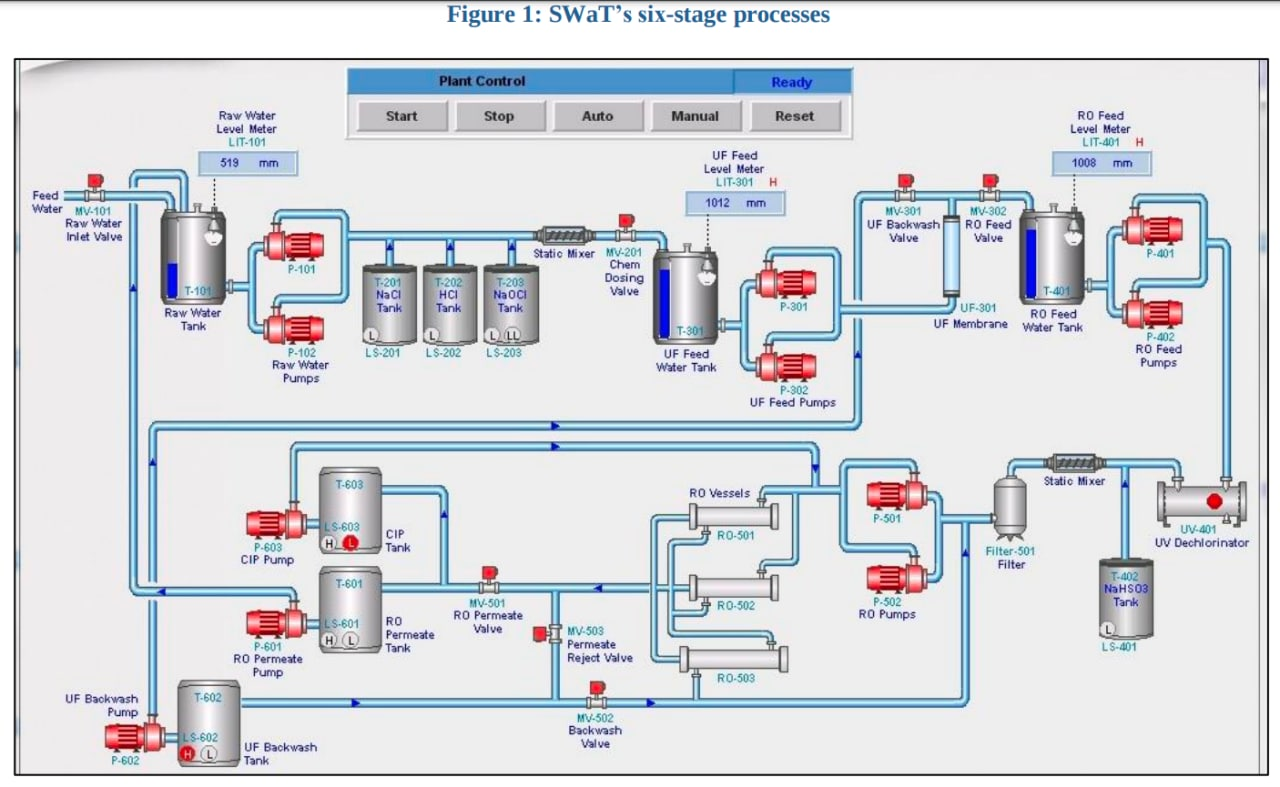
\includegraphics[scale=0.3]{swat_schema_2}
	\caption{SWaT schema}
	\label{fig:Schema SWaT}
\end{figure}

\begin{table}
	\centering
	\begin{tabular}{||c c c c||} 
		\hline
		Col1 & Col2 & Col2 & Col3 \\ [0.5ex] 
		\hline
		 & & & \\
		1 & 6 & 87837 & 787 \\ 
		2 & 7 & 78 & 5415 \\
		3 & 545 & 778 & 7507 \\
		4 & 545 & 18744 & 7560 \\
		5 & 88 & 788 & 6344 \\ [1ex] 
		\hline
	\end{tabular}
	\caption{This is the caption for the first table.}
	\label{table:1}
\end{table}
